\documentclass[portuguese]{textolivre}

% metadata
\journalname{Texto Livre}
\thevolume{18}
%\thenumber{1} % old template
\theyear{2025}
\receiveddate{\DTMdisplaydate{2024}{8}{31}{-1}}
\accepteddate{\DTMdisplaydate{2024}{12}{2}{-1}}
\publisheddate{\today}
\corrauthor{Márcio Nannini da Silva Florêncio}
\articledoi{10.1590/1983-3652.2025.54310}
%\articleid{NNNN} % if the article ID is not the last 5 numbers of its DOI, provide it using \articleid{} commmand 
% list of available sesscions in the journal: articles, dossier, reports, essays, reviews, interviews, editorial
\articlesessionname{articles}
\runningauthor{Florêncio, Sousa, Costa}
%\editorname{Leonardo Araújo} % old template
\sectioneditorname{Daniervelin Pereira}
\layouteditorname{João Mesquita}

\title{Perfil dos grupos de pesquisa no Piauí: entrelaçando linhas de saberes}
\othertitle{Profile of research groups in Piauí: intertwining lines of knowledge}

\author[1]{Márcio Nannini da Silva Florêncio~\orcid{0000-0001-5557-4181}\thanks{Email: \href{mailto:marcio.florencio@ifpi.edu.br}{marcio.florencio@ifpi.edu.br}}}
\author[2]{Romario Martins de Sousa~\orcid{0000-0001-6305-3511}\thanks{Email: \href{mailto:romariomartins@ifpi.edu.br}{romariomartins@ifpi.edu.br}}}
\author[3]{Benedita Marta Gomes Costa~\orcid{0000-0002-2740-0560}\thanks{Email: \href{mailto:martagcosta578@gmail.com}{martagcosta578@gmail.com}}}
\affil[1]{Instituto Federal do Piauí, Curso de Administração, Uruçuí, PI, Brasil.}
\affil[2]{Instituto Federal do Piauí, Coordenação Pedagógica, Uruçuí, PI, Brasil.}
\affil[3]{Universidade Estadual Vale do Acaraú, Curso de Administração, Sobral, CE, Brasil.}

\addbibresource{article.bib}
\usepackage{multirow}
\usepackage{array}

\begin{document}
\maketitle
\begin{polyabstract}
\begin{abstract}
Este artigo analisa o perfil dos grupos de pesquisa no Piauí, visando identificar elementos que possam fortalecer as atividades de Ciência, Tecnologia e Inovação (CT\&I) na região. Os dados foram coletados no Diretório dos Grupos de Pesquisa do CNPq entre março e maio de 2023. A pesquisa revelou a existência de 670 grupos distribuídos entre a UFPI, UESPI, IFPI e UFDPar, abordando aspectos como formação de recursos humanos, contexto geográfico, grandes áreas do conhecimento e parcerias. Os resultados indicam um crescimento constante no número de grupos, baixa inserção de técnicos e colaboradores internacionais e uma quantidade significativa de grupos com características atípicas. Observou-se também uma concentração dos grupos na região metropolitana de Teresina e no litoral do estado, destacando a necessidade de políticas de interiorização do ensino superior e da pesquisa. O estudo sugere a ampliação de investimentos em recursos humanos técnicos para melhorar o suporte e gestão dos laboratórios e atividades de pesquisa. A literatura destaca que a participação em grupos de pesquisa é crucial para a produtividade científica e o treinamento eficaz na pós-graduação, além de fomentar a socialização entre cientistas e a construção de valores e normas acadêmicas. Com base nesses achados, recomenda-se a continuidade e expansão das políticas que promovam a interiorização da pesquisa e a formação de grupos que atendam às demandas locais e regionais, contribuindo para o desenvolvimento científico e tecnológico do estado.

\keywords{Linhas de Pesquisas \sep Recursos Humanos \sep Cenário Estadual \sep Pesquisa e Desenvolvimento \sep Ciência e Tecnologia}
\end{abstract}

\begin{english}
\begin{abstract}
This article analyzes the profile of research groups in Piauí, aiming to identify elements that can strengthen Science, Technology, and Innovation (ST\&I) activities in the region. Data were collected from the CNPq Research Group Directory between March and May 2023. The research revealed the existence of 670 groups distributed among UFPI, UESPI, IFPI, and UFDPar, addressing aspects such as human resource development, geographic context, major areas of knowledge, and partnerships. The results indicate steady growth in the number of groups, low involvement of technical staff and international collaborators, and a significant number of groups with atypical characteristics. A concentration of groups was also observed in the metropolitan region of Teresina and the state’s coastal area, highlighting the need for policies to internalize higher education and research. The study suggests increasing investments in technical human resources to enhance the support and management of laboratories and research activities. The literature emphasizes that participation in research groups is crucial for scientific productivity and effective postgraduate training, as well as fostering socialization among scientists and the construction of academic values and norms. Based on these findings, it is recommended to continue and expand policies that promote the internalization of research and the formation of groups that meet local and regional demands, contributing to the state’s scientific and technological development.

\keywords{Research Lines \sep Human Resources \sep State Scenario \sep Research \& Development \sep Science \& Technology}
\end{abstract}
\end{english}
\end{polyabstract}

\section{Introdução}
\textcite{etzkowitz1993} destaca que a participação e colaboração em grupos de pesquisa são motores essenciais para a produtividade científica e para a formação eficaz na pós-graduação. Nesse contexto, \textcite{lopez2015,erdmann2013} afirmam que os grupos de pesquisa, atuando em áreas específicas do conhecimento, reúnem cientistas com interesses em pesquisas e discussões teórico-metodológicas semelhantes. Além de funcionar como um mecanismo de socialização, esses grupos são espaços onde valores, significados culturais e normas sociais de uma disciplina ou campo de pesquisa são construídos e difundidos pelos participantes, com diferentes níveis de experiência e conhecimento.

Complementarmente, \textcite{erdmann2013} argumentam que os grupos de pesquisa, organizados em equipes compostas por pesquisadores seniores e em formação, são fundamentais para a produção de novos conhecimentos científicos e tecnológicos. Esses grupos podem se estruturar em laboratórios fechados, como aqueles voltados para pesquisas clínicas, experimentais ou de desenvolvimento de produtos, ou em laboratórios abertos ou de campo, geralmente associados à pesquisa social.

No Brasil, os grupos de pesquisa estão cadastrados em uma base de dados organizada pelo Conselho Nacional de Desenvolvimento Científico e Tecnológico (CNPq). Criado em 1993, o Diretório dos Grupos de Pesquisa (DGP) serve como um inventário centralizado dos grupos de pesquisa científica e tecnológica em atividade no país, reunindo informações detalhadas sobre os pesquisadores, estudantes, técnicos, linhas de pesquisa, produção científica, tecnológica e artística, entre outros \cite{chiarini2022}.

Para que um grupo de pesquisa seja incluído no DGP, ele deve atender a certas características essenciais. Deve ser composto por um conjunto de indivíduos organizados hierarquicamente em torno de uma ou, eventualmente, duas lideranças (líder e vice-líder), podendo incluir apenas um único pesquisador e seus estudantes. O \textcite{cnpq2023b} destaca ainda que esses grupos devem apresentar uma hierarquia fundamentada na experiência, no destaque e na liderança científica ou tecnológica, envolvimento profissional permanente com atividades de pesquisa, organização em torno de linhas de pesquisa comuns e compartilhamento de instalações e equipamentos.

Atualmente, cabe ao dirigente institucional a responsabilidade de certificar os grupos de pesquisa cadastrados pelos pesquisadores em cada instituição. Nesse processo, o pesquisador líder deve fornecer informações detalhadas sobre o grupo, como sua identificação, linhas de pesquisa, líderes, recursos humanos, parcerias institucionais, equipamentos e \textit{softwares} relevantes. A certificação depende da completude das informações e da ausência de atipicidades. Grupos considerados atípicos podem apresentar características como a falta de estudantes ou técnicos, excesso de pesquisadores ou linhas de pesquisa, ausência de doutores, ou participação do líder em múltiplos grupos. Para mitigar o número de grupos atípicos, muitas instituições certificam apenas os grupos que solucionam as inconsistências identificadas durante o processo de validação. O \textcite{cnpq2023b} esclarece que a verificação dessas atipicidades visa orientar o pesquisador líder, sem acarretar prejuízos ou impedir a certificação.

Além disso, o líder do grupo deve atualizar as informações do grupo no mínimo a cada 12 meses. Grupos de pesquisa que não atualizam seus dados nesse período passam de "certificados" para "não atualizados" e, após mais 12 meses, são automaticamente excluídos da base de dados.

Diante desse cenário, o DGP emerge como um valioso ambiente de pesquisa, possibilitando a extração de dados para a construção de perfis dos grupos de pesquisa em níveis institucional, regional e nacional. A organização e análise desses dados constituem um estudo crucial para a otimização de recursos e o estímulo à colaboração entre pesquisadores e instituições, garantindo que as atividades de pesquisa estejam alinhadas com as demandas regionais. Considera-se que os grupos de pesquisa são espaços altamente propícios à produção de conhecimento científico e à formação de novos pesquisadores \cite{silva2020}.

No cenário acadêmico atual, as instituições públicas de ensino superior desempenham um papel fundamental na promoção e disseminação do conhecimento científico. Na região Nordeste do Brasil, características climáticas e indicadores socioeconômicos impulsionam pesquisas focadas em inovação, sustentabilidade, segurança hídrica, infraestrutura e desenvolvimento social e urbano, temas alinhados ao Plano Regional de Desenvolvimento do Nordeste \cite{brasil2020}. Nesse contexto, as instituições de ensino superior e de pesquisa são essenciais para estruturar iniciativas que auxiliem na formulação de políticas de Ciência, Tecnologia e Inovação (CT\&I).

Dentre os estados inseridos na região Nordeste, o Piauí contempla instituições públicas de ensino superior que desempenham um papel relevante no avanço da pesquisa científica, especialmente após a expansão dos espaços de pesquisa, a criação de fundações de amparo à pesquisa, o estímulo à pós-graduação \textit{stricto sensu} e o investimento de recursos públicos. Esses fatores têm promovido maior sinergia e continuidade na pesquisa científica, tecnológica e de inovação. Assim, é na perspectiva regional que a presente pesquisa propõe analisar o perfil dos grupos de pesquisa, tendo como base as instituições públicas de ensino superior sediadas no Piauí.

Nesta pesquisa foi possível verificar que o primeiro grupo de pesquisa no estado foi criado em 1991, na Universidade Federal do Piauí (UFPI), com foco nas ciências humanas, voltado para pesquisas arqueológicas no Norte do estado. Os primeiros trabalhos arqueológicos da UFPI, realizados no litoral do Piauí em 1995, foram conduzidos pelo extinto Núcleo de Estudos Históricos-Geográficos (NEHG), vinculado ao Departamento de Geografia e História (DGH/CCHL) \cite{silva2017}. Esse grupo foi pioneiro na área e possibilitou a publicação de achados significativos para a arqueologia local e regional, convergindo com a formação de recursos humanos por meio de cursos de pós-graduação \textit{stricto sensu} focados em estudos sobre arte rupestre, líticos, cerâmicos e bioarqueológicos nos principais Parques Nacionais do estado (Sete Cidades, Serra da Capivara e Serra das Confusões) e no litoral.

Neste cenário, ao delinear a evolução e a dinâmica do perfil desses grupos de pesquisa, este estudo apresenta não apenas o mapeamento das suas áreas de atuação, mas também um panorama detalhado da composição dos recursos humanos envolvidos. Dessa forma, busca-se fornecer uma visão abrangente das atividades de pesquisa desenvolvidas nas instituições públicas de ensino superior do Piauí, ressaltando a importância dos grupos de pesquisa na construção de uma base sólida para o avanço científico e tecnológico das instituições onde atuam.

\section{Fortalecimento da Ciência, Tecnologia e Inovação (C,T\&I) por meio dos grupos de pesquisa}
Grupos de pesquisa desempenham um papel essencial no fortalecimento das atividades de CT\&I, promovendo sinergias entre universidades, empresas e governo. Essas colaborações são particularmente significativas em contextos regionais, que muitas vezes são caracterizados por estruturas específicas relacionadas àquela região e que demandam soluções adaptadas às suas particularidades. Essas interações permitem a transferência de tecnologia, a cocriação de conhecimento e o compartilhamento de recursos, criando um ambiente propício ao desenvolvimento de inovações alinhadas às demandas do mercado e às prioridades regionais \cite{florencio2018}. 

A literatura internacional destaca o impacto positivo dos grupos de pesquisa na dinâmica da inovação. Um estudo conduzido na Colômbia evidencia que a implementação de um plano de gestão do conhecimento é essencial para integrar pesquisa e inovação em grupos de pesquisa universitários \cite{paezlogreira2016}. Esses grupos constituem a base do trabalho de pesquisa universitário e são as principais fontes de resultados inovadores, contribuindo de forma significativa para o desenvolvimento socioeconômico regional e nacional \cite{cabeza-pulles2018}. Além disso, essas iniciativas não apenas impulsionam o desenvolvimento tecnológico, mas também contribuem para a formação de capital humano qualificado, essencial para sustentar avanços em CT\&I \cite{munoz2024}.

No Brasil, estudos têm destacado as contribuições dos grupos de pesquisa para o fortalecimento da produção científica e tecnológica em Instituições Científicas e Tecnológicas públicas. Esses grupos disseminam conhecimento por meio de eventos científicos, publicações em periódicos, livros e capítulos de livros. Embora em menor escala, observa-se também a produção tecnológica, como novos produtos, processos e softwares, evidenciando a necessidade de intensificar esforços em inovação tecnológica no país \cite{lino2010,perucchi2011}.

Ademais, \textcite{souza2024} destacam a importância de desenvolver a capacidade absortiva – tanto potencial quanto realizada – dos grupos de pesquisa no Piauí. Para os autores, esses grupos devem adquirir, assimilar, transformar e aplicar conhecimentos externos valiosos gerando inovações. Para isso, é fundamental que os líderes adotem rotinas e processos que garantam a contínua renovação do estoque de conhecimento, promovendo resultados concretos de inovação.

\section{Metodologia}\label{sec-fmt-manuscrito}
A pesquisa documental conduzida pode ser classificada como um estudo descritivo com abordagem quantitativa, centrado na análise das informações coletadas. O percurso metodológico foi organizado em duas etapas principais: (i) fonte de dados e estratégia de busca; e (ii) variáveis adotadas e procedimentos de análise dos dados.

Em relação às fontes de dados e à estratégia de busca, o mapeamento dos grupos de pesquisa das Instituições de Ensino Superior (IES) públicas do Piauí foi realizado a partir do DGP da Plataforma Lattes \cite{cnpq2023a}. Esse diretório oferece uma lista detalhada de informações sobre os grupos de pesquisa no país \cite{florencio2018}. A busca foi realizada no sítio eletrônico do \textcite{cnpq2023a} utilizando os seguintes filtros: “Região: Nordeste”, “UF: Piauí”, “Instituição: Instituto Federal do Piauí”, “Instituição: Universidade Estadual do Piauí”, “Instituição: Universidade Federal do Piauí” e “Instituição: Universidade Federal do Delta do Parnaíba”. Vale destacar que, conforme a estratégia de pesquisa adotada, não foi possível identificar grupos de pesquisa vinculados à Universidade Federal do Vale do São Francisco, que possui um campus no município de São Raimundo Nonato, Piauí.

A seleção das instituições teve como objetivo incluir as IES públicas situadas no Piauí. Este recorte se justifica pelo papel fundamental que essas instituições desempenham na geração e disseminação do conhecimento para a sociedade, atuando como agentes de inovação no contexto em que estão inseridas \cite{tosta2016}. Além disso, as universidades públicas participam ativamente em atividades de inovação e transferência de conhecimento e tecnologia, figurando entre os principais depositantes de patentes de invenção no Instituto Nacional da Propriedade Industrial (INPI) \cite{closs2012,inpi2020}.

Devido às limitações da base de dados, os grupos de cada IES pública foram recuperados individualmente. Posteriormente, as informações coletadas foram exportadas e organizadas em planilhas no software Microsoft Excel. A coleta dos dados ocorreu manualmente entre março e maio de 2023. Não foram aplicadas restrições quanto às áreas de conhecimento ou ao período de criação dos grupos, visando obter uma visão abrangente da amostra estudada. Como resultado, foram identificados 679 grupos de pesquisa vinculados às IES públicas do Piauí. Destes, 9 laboratórios foram removidos por estarem excluídos ou duplicados, resultando em 670 grupos de pesquisa válidos. Convém ressaltar que, segundo o \textcite{cnpq2023b}, os dados de grupos de pesquisa podem desaparecer por razões como: (i) troca do primeiro líder do grupo; (ii) retirada da certificação pelo dirigente de pesquisa da instituição; (iii) exclusão do grupo pelo próprio líder; e (iv) exclusão automática pelo sistema após mais de 24 meses sem atualização.

Quanto às variáveis adotadas e aos procedimentos de análise dos dados, os dados coletados no diretório dos grupos de pesquisa do CNPq foram tratados e analisados utilizando o \textit{software} Microsoft Excel. As variáveis consideradas incluíram nome do grupo, ano de formação, áreas predominante e específica, instituição, linhas de pesquisa, número de pesquisadores, técnicos e estudantes, formação dos membros e parcerias. Com essas variáveis definidas, utilizou-se a estatística descritiva simples para analisar e interpretar o conjunto de dados recuperados, observando-se as frequências absolutas e relativas.


\section{Resultados e discussão}\label{sec-formato}

\subsection{Perfil dos grupos de pesquisa das IES públicas do Piauí}\label{sec-modelo}
Este tópico apresenta o perfil dos grupos de pesquisa das IES públicas do Piauí, com base nas informações obtidas do DGP do CNPq. De acordo com \textcite{cezar2018}, analisar essas informações é essencial para entender os limites e o perfil geral da atividade científica e tecnológica no contexto investigado. Neste estudo, foram analisados 670 grupos de pesquisa vinculados às IES públicas do estado.

A \Cref{fig1} mostra a evolução temporal da formação desses grupos de pesquisa no período de 1991 a 2023. O primeiro grupo de pesquisa, criado em 1991, focou no cadastramento de sítios arqueológicos, nas ocupações humanas pré-históricas no Norte do Piauí e na conservação de arte rupestre. Ele pertence à área de arqueologia e está vinculado à UFPI.

\begin{figure}
\centering
\begin{minipage}{.75\textwidth}
    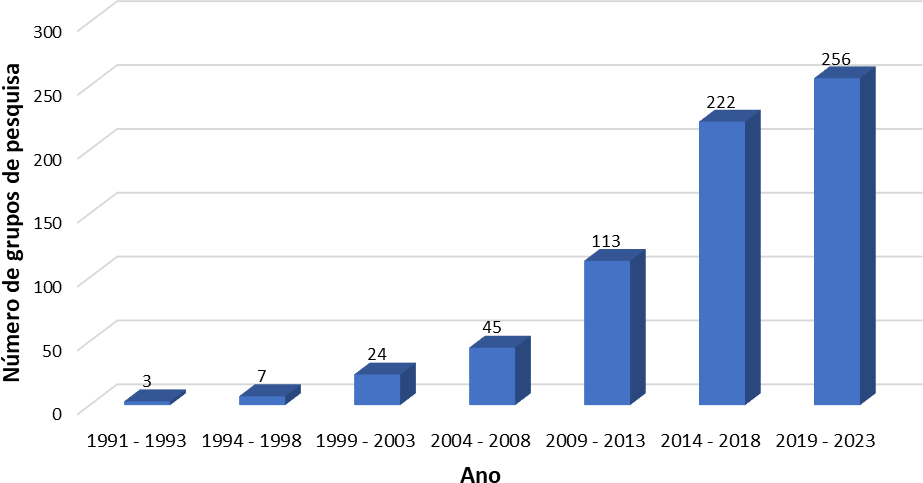
\includegraphics[width=\linewidth]{Fig1.png}
    \caption{Evolução temporal do ano de criação dos grupos de pesquisa no Piauí (1991 - 2023)}
    \label{fig1}
    \source{Elaborado pelos autores a partir do DGP/CNPq (2023a).}
\end{minipage}
\end{figure}

Entre 1991 e 1998, o número de grupos de pesquisa foi baixo, com apenas 10. No entanto, houve um crescimento acentuado nos períodos mais recentes: de 2014 a 2018 foram formados 222 grupos (33,1\%) e de 2019 a 2023, 256 grupos (38,2\%). A taxa de crescimento anual foi de aproximadamente 9,3\% entre 1994 e os primeiros meses de 2023. Destaca-se que 88,2\% dos grupos de pesquisa foram criados entre 2009 e 2023. Como os dados foram coletados em março de 2023, espera-se um aumento ainda maior nesse ano. Esse crescimento pode ser atribuído à expansão dos programas de pós-graduação, aos investimentos em pesquisa e à obrigatoriedade de cadastro na Plataforma Lattes \cite{costa2014,nickel2016}.

Analisando os Planos de Desenvolvimento Institucional (PDIs) das instituições pesquisadas, observou-se um aumento substancial nos programas de pós-graduação \textit{stricto sensu}. Em 2015, a UFPI tinha 37 programas de mestrado e 7 de doutorado, que cresceram para 46 programas de mestrado e 21 de doutorado até o final de 2019 \cite{ufpi2015pdi,ufpi2020pdi}. A Universidade Estadual do Piauí (UESPI) possuía 4 programas de mestrado em 2015 que foram ampliados para 8 até 2020. Em relação aos doutorados, a UESPI mantinha 3 programas, sendo dois na modalidade Doutorado Interinstitucional (DINTER) que foram preservados até 2023 \cite{uespi2017pdi,uespi2022pdi}. O Instituto Federal do Piauí (IFPI) oferece apenas programas de mestrado, sendo um acadêmico e 4 profissionais, com planos de expansão até 2024 \cite{ifpi2020}. A Universidade Federal do Delta do Parnaíba (UFDPar), criada em 2018 pela Lei nº 13.651, conta com 6 programas de mestrado e 1 programa de doutorado \cite{ufdpar2023pdi}.

Observa-se que 478 grupos de pesquisa (71,3\%) têm menos de 10 anos de atividade, enquanto 192 (28,7\%) têm 10 anos ou mais. Esses dados sugerem que a maioria dos grupos é relativamente recente em seu campo, enquanto uma minoria é considerada consolidada.

A \Cref{tbl1} detalha o número de grupos de pesquisa, linhas de pesquisa e colaboradores por município no Piauí com IES públicas. Esses grupos reúnem 5.478 pesquisadores (44,5\%), 6.623 alunos (53,8\%), 136 técnicos (1,1\%) e 69 colaboradores estrangeiros (0,6\%), totalizando 12.306 membros envolvidos em 2.237 linhas de pesquisa.

\begin{table}[htbp]
\centering
\begin{threeparttable}
\caption{Número de grupos de pesquisa, linhas de pesquisa, pesquisadores, alunos, técnicos e colaboradores estrangeiros por município do Piauí.}
\label{tbl1}
\begin{tabular}{lllllll}
\toprule
Município & G & L & A & T & P & E \\ 
\midrule
Teresina & 406 & 1339 & 4290 & 60 & 3435 & 58 \\
Parnaíba & 91 & 292 & 712 & 13 & 553 & 5 \\
Picos & 51 & 185 & 622 & 27 & 398 & 0 \\
Floriano & 29 & 94 & 359 & 6 & 273 & 4 \\
Bom Jesus & 25 & 88 & 260 & 14 & 199 & 0 \\
Piripiri & 14 & 48 & 78 & 3 & 132 & 0 \\
Corrente & 10 & 22 & 43 & 3 & 78 & 0 \\
Uruçuí & 8 & 39 & 63 & 2 & 126 & 1 \\
Campo Maior & 6 & 22 & 54 & 1 & 51 & 0 \\
Paulistana & 6 & 23 & 18 & 1 & 38 & 0 \\
Oeiras & 5 & 14 & 37 & 0 & 28 & 0 \\
São Raimundo Nonato & 5 & 16 & 25 & 0 & 41 & 0 \\
Pedro II & 4 & 17 & 18 & 1 & 37 & 0 \\
Valença do Piauí & 4 & 14 & 12 & 3 & 36 & 1 \\
Angical & 3 & 7 & 22 & 2 & 24 & 0 \\
Barras & 1 & 4 & 1 & 0 & 6 & 0 \\
Cocal & 1 & 9 & 0 & 0 & 19 & 0 \\
São João do Piauí & 1 & 3 & 9 & 0 & 4 & 0 \\
\midrule
Total & 670 & 2236 & 6623 & 136 & 5478 & 69 \\
\bottomrule
\end{tabular}
\begin{tablenotes}
\footnotesize{
\item{G = Número de grupos de pesquisa;}
\item{L = Número de linhas de pesquisa;} 
\item{A = Número de alunos;}
\item{T = Número de técnicos;}
\item{P = Número de Pesquisadores;}
\item{E = Número de colaboradores estrangeiros.}
}
\end{tablenotes}
\source{Elaborado pelos autores a partir do \textcite{cnpq2023a}.}
\end{threeparttable}
\end{table}

%Ver se há problema no código da nota

Nos grupos de pesquisa, observa-se a ausência de técnicos na maioria (87,6\%), totalizando 587 grupos sem esses profissionais. \textcite{nickel2016} destacam que técnicos são essenciais para manter recursos físicos e integrar pesquisa e ensino, contribuindo conforme sua especialização. \textcite{vilarino2017} alertam que a falta de técnicos sobrecarrega os demais membros, comprometendo a eficiência dos grupos.

A presença de técnicos nas instituições de ensino superior está geralmente vinculada a laboratórios de ensino/pesquisa. É comum a contratação de profissionais especializados para o manejo de materiais e equipamentos. As chamadas públicas para contratação de técnicos estão frequentemente vinculadas a cursos dessas áreas, com ofertas de vagas para cargos como Técnico de Nível Médio em diversas especialidades, tais como Auxiliar de Serviço Bucal, Programador Visual, Técnico de Laboratório, Técnico em Audiovisual e Analista de Tecnologia da Informação, entre outros.

No entanto, é pertinente ressaltar que, ao assumirem suas funções, esses técnicos nem sempre são integrados às atividades de pesquisa, sendo muitas vezes alocados em setores administrativos, sem colaboração direta com os pesquisadores.

Nesse cenário, cursos das áreas de Ciência da Saúde e Ciências Agrárias tendem a contar com um maior número de técnicos, seguidos por Ciências Humanas e Ciências Sociais Aplicadas, conforme observado nas \Cref{tbl2,tbl6,tbl8} deste estudo. Em outras áreas, pesquisadores dependem de apoio administrativo para tarefas como organização de dados e prestação de contas, embora esses profissionais não sejam formalmente classificados como técnicos nos grupos.

Correspondendo a um total de 60,6\% dos grupos cadastrados no CNPq, o município de Teresina dispõe do maior número de grupos no estado e detém os maiores números de colaboradores, abrangendo aproximadamente 62,0\% dos pesquisadores, 64,8\% dos alunos, 44,1\% dos técnicos e 84,1\% dos pesquisadores estrangeiros. O município também possui o maior número de linhas de pesquisa (59,9\%), distribuídas por todas as grandes áreas do conhecimento.

Parnaíba ocupa a segunda posição com 91 grupos de pesquisa (13,6\%), envolvendo 10,1\% dos pesquisadores, 10,8\% dos alunos, 9,6\% dos técnicos e 7,2\% dos colaboradores estrangeiros, distribuídos em 292 linhas de pesquisa (13,1\%). Picos está em terceiro lugar com 51 grupos (7,6\%), reunindo 7,3\% dos pesquisadores, 9,4\% dos alunos, 19,9\% dos técnicos e nenhum colaborador estrangeiro, atuando em 185 linhas de pesquisa (8,3\% do total estadual).

Entre os 18 municípios com grupos vinculados às IES públicas, Barras (IFPI), Cocal (UFPI, UESPI, IFPI) e São João do Piauí (IFPI) registraram apenas um grupo cadastrado no DGP/CNPq. Destaca-se Cocal com 19 pesquisadores em seu único grupo dedicado à agronomia.
Além de Teresina e Parnaíba, Floriano, Uruçuí e Valença do Piauí possuem colaboradores estrangeiros nas atividades científicas das IES locais. No entanto, os dados mostram a necessidade de ampliar a cooperação internacional nas quatro instituições analisadas (UFPI, UESPI, IFPI e UFDPar). \textcite{ramos2018} atribui a baixa internacionalização à ausência de estratégias nacionais e políticas institucionais adequadas, dificultando parcerias científicas duradouras.

Em relação ao número total de membros por município, Teresina lidera com 7.843 participantes, seguida por Parnaíba com 1.283 e Picos com 1.047. Os grupos variam de 1 a 145 membros, com média de 18 integrantes por grupo. \textcite{verbree2011} destacam que grupos maiores produzem resultados significativos em linhas interdisciplinares, enquanto grupos menores abordam tópicos mais restritos, sendo mais fáceis de gerenciar e menos onerosos em termos de coordenação.

Destacam-se algumas atipicidades entre os grupos de pesquisa das IES públicas do Piauí, como: 1,3\% dos grupos são formados por apenas um pesquisador; 7,8\% não possuem estudantes; 87,6\% não têm técnicos; 24,9\% têm mais de dez pesquisadores; e 1,5\% possuem mais de dez linhas de pesquisa. Esses dados são semelhantes aos observados por \textcite{miano2020} nas instituições federais de educação do Rio de Janeiro.

A ausência de estudantes nos grupos de pesquisa é considerada preocupante por \textcite{costa2014,erdmann2017}, que alertam para a perda de oportunidades de engajar futuros pesquisadores, que, por sua vez, poderiam possibilitar o robustecimento da pesquisa e da produção científica e assim beneficiar diretamente o ensino no país.

Sobre a distribuição dos grupos de pesquisa por IES (\Cref{tbl2}), observa-se que a maioria está vinculada à Universidade Federal do Piauí (UFPI) com 60\%, seguida pela UESPI com 22\%, IFPI com 11\% e UFDPar com 6,7\%.

A UFPI destaca-se pela ampla participação em grupos de pesquisa no estado, impulsionada por atividades que integram docentes, técnicos, graduandos e pós-graduandos, com estratégias metodológicas éticas e consistentes para a produção do conhecimento \cite{ufpi2020pdi}. A instituição também fomenta a formação e o fortalecimento de grupos intra e interdisciplinares, promovendo colaborações nacionais e internacionais e a inclusão de professores com diferentes perfis acadêmicos \cite{ufpi2020pdi}.

Com base na \Cref{tbl2}, verifica-se que as áreas de Ciências Humanas, Ciências da Saúde e Ciências Sociais Aplicadas apresentam os maiores percentuais de grupos no Piauí (23,6\%, 16,6\% e 15,4\%, respectivamente), enquanto as áreas de Engenharias e outras apresentam os menores percentuais, com 4,3\% e 1,9\%, respectivamente.

Nota-se também que a distribuição desses grupos entre as IES públicas no Piauí varia conforme a vocação institucional e a oferta de cursos de graduação e programas de pós-graduação \textit{stricto sensu} em cada área. No caso da UFPI, as áreas de Ciências Humanas (14\%), Ciências da Saúde (11,6\%) e Ciências Sociais Aplicadas (8,4\%) concentram os maiores percentuais de grupos ativos, enquanto as áreas de Linguística, Letras e Artes (2,8\%) e “outras” (0,4\%) apresentam os menores percentuais.

Na UESPI, as Ciências Humanas (6,6\%), Ciências da Saúde (3,4\%) e Linguística, Letras e Artes (3,3\%) lideram em número de grupos de pesquisa, ao passo que Engenharias (0,4\%) e “outras” (0,4\%) têm os menores valores. É importante destacar que a UESPI possui o maior número de grupos de pesquisa na área de Linguística, Letras e Artes em comparação com as demais IES públicas do Piauí. Esse desempenho pode ser atribuído à consolidação de dois programas de mestrado na área de Letras, um acadêmico e outro profissional, além de um DINTER em Linguística com a Universidade de São Paulo \cite{uespi2022pdi}.

\begin{table}[htbp]
\centering
\begin{threeparttable}
\caption{Número de grupos de pesquisa por IES e grande área do conhecimento no Piauí.}
\label{tbl2}
\begin{tabular}{llll}
\toprule
IES & Grande Área do Conhecimento & n & \% \\ 
\midrule
\multirow{9}{*}{UFPI} & Ciências Agrárias & 46 & 6,9\% \\
 & Ciências Biológicas & 40 & 6,0\% \\
 & Ciências da Saúde & 78 & 11,6\% \\
 & Ciências Exatas e da Terra & 46 & 6,9\% \\
 & Ciências Humanas & 94 & 14,0\% \\
 & Ciências Sociais Aplicadas & 56 & 8,4\% \\
 & Engenharias & 20 & 3,0\% \\
 & Linguística, Letras e Artes & 19 & 2,8\% \\
 & Outra & 3 & 0,4\% \\
\midrule
Subtotal & & 402 & 60,0\% \\
\midrule
\multirow{9}{*}{UESPI} & Ciências Agrárias & 9 & 1,3\% \\
 & Ciências Biológicas & 14 & 2,1\% \\
 & Ciências da Saúde & 23 & 3,4\% \\
 & Ciências Exatas e da Terra & 11 & 1,6\% \\
 & Ciências Humanas & 44 & 6,6\% \\
 & Ciências Sociais Aplicadas & 20 & 3,0\% \\
 & Engenharias & 3 & 0,4\% \\
 & Linguística, Letras e Artes & 22 & 3,3\% \\
 & Outra & 3 & 0,4\% \\
\midrule
Subtotal & & 149 & 22,2\% \\
\midrule
\multirow{9}{*}{IFPI} & Ciências Agrárias & 7 & 1,0\% \\
 & Ciências Biológicas & 4 & 0,6\% \\
 & Ciências da Saúde & 1 & 0,1\% \\
 & Ciências Exatas e da Terra & 19 & 2,8\% \\
 & Ciências Humanas & 11 & 1,6\% \\
 & Ciências Sociais Aplicadas & 15 & 2,2\% \\
 & Engenharias & 6 & 0,9\% \\
 & Linguística, Letras e Artes & 4 & 0,6\% \\
 & Outra & 7 & 1,0\% \\
\midrule
Subtotal & & 74 & 11,0\% \\
\midrule
\multirow{9}{*}{UFDPar} & Ciências Agrárias & 1 & 0,1\% \\
 & Ciências Biológicas & 9 & 1,3\% \\
 & Ciências da Saúde & 9 & 1,3\% \\
 & Ciências Exatas e da Terra & 3 & 0,4\% \\
 & Ciências Humanas & 9 & 1,3\% \\
 & Ciências Sociais Aplicadas & 12 & 1,8\% \\
 & Engenharias & 0 & 0,0\% \\
 & Linguística, Letras e Artes & 2 & 0,3\% \\
 & Outra & 0 & 0,0\% \\
\midrule
Subtotal & & 45 & 6,7\% \\
\midrule
Total & & 670 & 100,0\% \\
\bottomrule
\end{tabular}
\source{Elaborado pelos autores a partir do \textcite{cnpq2023a}.}
\end{threeparttable}
\end{table}

O IFPI, por sua vez, concentra os maiores números de grupos de pesquisa nas áreas de Ciências Exatas e da Terra (2,8\%) e Ciências Sociais Aplicadas (2,2\%). Em contrapartida, Ciências da Saúde (0,1\%), Ciências Biológicas (0,6\%) e Linguística, Letras e Artes (0,6\%) têm os menores percentuais. Esses números refletem a missão da rede federal de ensino, conforme estabelecido pela Lei nº 11.892 de 29 de dezembro de 2008, que orienta o IFPI a se constituir como um centro de excelência na oferta de ensino em ciências, com ênfase em ciências aplicadas, além de promover programas especiais de formação pedagógica para professores da educação básica, especialmente nas áreas de ciências e matemática \cite{brasil2008}.

Destaca-se que o IFPI oferece 47 cursos de Administração, sendo 38 técnicos e 9 superiores, além de 24 cursos de licenciatura nas áreas de matemática, física e química, distribuídos por municípios como Angical do Piauí, Cocal, Corrente, Campo Maior, Floriano, Oeiras, Picos, Parnaíba, Paulistana, Piripiri, São Raimundo Nonato, Teresina, Valença do Piauí e Uruçuí \cite{ifpi2020}.

A UFDPar concentra os maiores percentuais de grupos de pesquisa em Ciências Sociais Aplicadas (1,8\%), Ciências da Saúde (1,3\%) e Ciências Biológicas (1,3\%), enquanto Ciências Agrárias (0,1\%) e Linguística, Letras e Artes (0,3\%) têm os menores percentuais. A UFDPar oferece 12 cursos superiores, incluindo biomedicina, medicina, administração, turismo e engenharia de pesca, além de 6 programas de mestrado em áreas como saúde da família, biotecnologia e psicologia, e 1 doutorado em biotecnologia.

Segundo \textcite{florencio2018}, a cooperação acadêmica entre os grupos de pesquisa é crucial para o desenvolvimento de pesquisas, especialmente diante das limitações orçamentárias e de infraestrutura das IES públicas. De acordo com a \Cref{tbl3}, as áreas com o maior número de grupos de pesquisa com parcerias interinstitucionais são Ciências Humanas (21,2\%), Ciências Biológicas (16,5\%) e Ciências Agrárias (15,9\%), enquanto Engenharias (2,9\%) e “outras” (1,2\%) apresentam os menores percentuais de cooperação.

\begin{table}[htbp]
\centering
\begin{threeparttable}
\caption{Número de grupos de pesquisa com interação com outras instituições por grande área do conhecimento.}
\label{tbl3}
\begin{tabular}{lccc}
\toprule
Grande Área do Conhecimento & n & \% & Nº de parceiros\\ 
 \midrule
Ciências Humanas & 36 & 21,2\% & 73 \\
Ciências Biológicas & 28 & 16,5\% & 74 \\
Ciências Agrárias & 27 & 15,9\% & 61 \\
Ciências da Saúde & 25 & 14,7\% & 49 \\
Ciências Exatas e da Terra & 19 & 11,2\% & 43 \\
Ciências Sociais Aplicadas & 15 & 8,8\% & 26 \\
Linguística, Letras e Artes & 13 & 7,6\% & 26 \\
Engenharias & 5 & 2,9\% & 18 \\
Outra & 2 & 1,2\% & 2 \\
\midrule
Total & 170 & 100,0\% & 225 \\
\bottomrule
\end{tabular}
\source{Elaborado pelos autores a partir do \textcite{cnpq2023a}.}
\end{threeparttable}
\end{table}

Os grupos de pesquisa com parcerias institucionais possuem de 1 a 14 parceiros, com média de 2 por grupo, destacando-se as áreas de Ciências Humanas, Ciências Biológicas e Ciências Agrárias. No entanto, 74,6\% dos grupos (cerca de 500) não possuem parcerias.

Estudando a colaboração universidade-empresa em Sergipe, \textcite{florencio2018} identificaram que a maioria dos grupos interage mais com instituições de ensino, especialmente universidades. Áreas como Ciências Biológicas, Engenharias, Ciências da Saúde e Ciências Agrárias colaboram mais com empresas devido à aplicação prática de suas pesquisas. Essa colaboração entre universidade e empresa ocorre frequentemente no sentido de as universidades buscarem as empresas para o fornecimento de insumos, enquanto as empresas procuram as universidades para o desenvolvimento de projetos de pesquisa e transferência de tecnologia.

\subsection{Grupos de pesquisa por área do conhecimento: tecendo linhas de saberes no Piauí}\label{sec-organizacao}
A \Cref{tbl4} apresenta o número de grupos de pesquisa e seus membros na grande área de Ciências Agrárias no Piauí. Observa-se que a UFPI lidera em número de grupos de pesquisa nessa área, com um total de 995 membros, distribuídos entre docentes (39\%), alunos (58,8\%), técnicos (2\%) e colaboradores estrangeiros (0,2\%).

\begin{table}[htbp]
\caption{Número de grupos de pesquisa, pesquisadores, alunos, técnicos e colaboradores estrangeiros cadastrados por IES na área de Ciências Agrárias no Piauí (1994 a 2023).}
\label{tbl4}
\centering
\begin{tabular}{>{\raggedright\arraybackslash}p{5cm} l l l l}
\toprule
Área dos grupos de pesquisa/nº de grupos de pesquisa & UFPI & UESPI & IFPI & UFDPar \\ 
\midrule
\multicolumn{5}{c}{Ciências Agrárias} \\
\midrule
Agronomia & 15 & 7 & 2 & 0 \\
Ciência e Tec. de Alimentos & 3 & 0 & 3 & 1 \\
Engenharia Agrícola & 3 & 0 & 0 & 0 \\
Medicina Veterinária & 9 & 0 & 0 & 0 \\
Rec. Florestais e Eng. Florestal & 5 & 0 & 0 & 0 \\
Rec. Pesqueiros e Eng. de Pesca & 1 & 0 & 0 & 0 \\
Zootecnia & 10 & 2 & 2 & 0 \\
\midrule
Subtotal & 46 & 9 & 7 & 1 \\
\midrule
Nº de pesquisadores & 388 & 72 & 60 & 10 \\
Nº de alunos & 585 & 102 & 34 & 4 \\
Nº de técnicos & 20 & 4 & 1 & 0 \\
Nº de colaboradores estrangeiros & 2 & 0 & 0 & 0 \\
\bottomrule
\end{tabular}
\source{Elaborado pelos autores a partir do \textcite{cnpq2023a}.}
\end{table}

As subáreas de Agronomia, Zootecnia e Medicina Veterinária concentram o maior número de grupos de pesquisa, enquanto Engenharia Agrícola e Recursos Pesqueiros/Engenharia de Pesca têm pouca representatividade (\Cref{tbl4}). Em termos de temas de pesquisa, destacam-se solos, fitotecnia e tecnologia de sementes (agronomia), sanidade e reprodução animal (medicina veterinária) e análise de alimentos e forragicultura (zootecnia).

A área de Ciências Agrárias no Piauí reúne 1.282 membros, sendo 530 pesquisadores, 725 alunos, 25 técnicos e 2 colaboradores estrangeiros em IES públicas. Agronomia é a única subárea presente em todas as IES públicas, enquanto Engenharia Agrícola, Medicina Veterinária, Recursos Florestais/Engenharia Florestal e Recursos Pesqueiros/Engenharia de Pesca não possuem grupos ativos na UESPI, IFPI e UFDPar. A UFDPar e o IFPI apresentam os menores números de grupos na área.

\textcite{sena2020} destacam a importância dos grupos de pesquisa na formação acadêmica e profissional em Ciências Agrárias, ao integrar teoria, troca de experiências e atividades científicas, promovendo conhecimento específico e desenvolvimento integral dos participantes.
Já a área de Ciências Biológicas lidera em diversidade de subáreas entre as grandes áreas do conhecimento (\Cref{tbl5}).

\begin{table}[htbp]
\centering
\begin{threeparttable}
\caption{Número de grupos de pesquisa, pesquisadores, alunos, técnicos e colaboradores estrangeiros cadastrados por IES na área de Ciências Biológicas no Piauí (1994 a 2023).}
\label{tbl5}
\begin{tabular}{>{\raggedright\arraybackslash}p{5cm} l l l l}
\toprule
Área dos grupos de pesquisa/nº de grupos de pesquisa & UFPI & UESPI & IFPI & UFDPar \\ 
\midrule
\multicolumn{5}{c}{Ciências Biológicas} \\
\midrule
Biofísica & 1 & 0 & 0 & 0 \\
Biologia Geral & 2 & 2 & 1 & 0 \\
Bioquímica & 1 & 0 & 0 & 0 \\
Biotecnologia & 1 & 0 & 0 & 2 \\
Botânica & 3 & 2 & 2 & 1 \\
Ecologia & 9 & 2 & 0 & 0 \\
Farmacologia & 5 & 0 & 0 & 2 \\
Fisiologia & 3 & 1 & 0 & 1 \\
Genética & 4 & 1 & 1 & 1 \\
Microbiologia & 1 & 1 & 0 & 1 \\
Morfologia & 4 & 0 & 0 & 0 \\
Parasitologia & 3 & 1 & 0 & 0 \\
Zoologia & 3 & 4 & 0 & 1 \\
\midrule
Subtotal & 40 & 14 & 4 & 9 \\
\midrule
Nº de pesquisadores & 288 & 116 & 17 & 66 \\
Nº de alunos & 497 & 120 & 30 & 125 \\
Nº de técnicos & 2 & 3 & 3 & 4 \\
Nº de colaboradores estrangeiros & 2 & 0 & 1 & 0 \\
\bottomrule
\end{tabular}
\source{Elaborado pelos autores a partir do \textcite{cnpq2023a}.}
\end{threeparttable}
\end{table}

A UFPI concentra a maior parte dos grupos de pesquisa na área de Ciências Biológicas, com 59,7\% dos grupos distribuídos em diversas subáreas. Em contraste, o IFPI possui o menor número, com apenas quatro grupos de pesquisa ativos, nas áreas de biologia geral, botânica e genética. As subáreas com mais grupos de pesquisa são botânica, ecologia e zoologia, enquanto biofísica, bioquímica e morfologia não possuem grupos ativos na UESPI, IFPI e UFDPar. As subáreas de botânica e genética estão presentes em todas as IES públicas. Entre os temas abordados nas linhas de pesquisa destacam-se o ensino de botânica, anatomia vegetal e taxonomia de plantas (botânica); conservação vegetal, conservação de espécies e herpetologia (ecologia); e ecologia e taxonomia de insetos (zoologia).

A área reúne 1.274 membros, sendo 487 pesquisadores, 772 alunos, 12 técnicos e 3 colaboradores estrangeiros. Costa, Pedro e Macedo (2013) destacaram a escassez de alunos e técnicos em genética, problema mitigado pelo aumento de cursos de graduação e pós-graduação, embora o número de técnicos permaneça baixo.

Na grande área de Ciências da Saúde (\Cref{tbl6}), a UFPI lidera com 70,3\% dos grupos de pesquisa, seguida pela UESPI (20,7\%) e o IFPI com apenas um grupo ativo. Enfermagem, saúde coletiva e fisioterapia concentram o maior número de grupos, enquanto farmácia e nutrição têm participação reduzida.

Para\textcite{costa2018}, o número expressivo de grupos de pesquisa em enfermagem deve-se à expansão dos programas de pós-graduação e ao crescente interesse dos estudantes, resultando em maior produção científica e avanços na área.

Entre os temas abordados nas Ciências da Saúde, destacam-se o processo de cuidar em saúde e enfermagem, prevenção e promoção da saúde, qualidade de vida de idosos, e tecnologias em saúde (enfermagem); epidemiologia e educação em saúde (saúde coletiva); e desempenho humano e avaliação em fisioterapia (fisioterapia e terapia ocupacional). Vale ressaltar a existência de um grupo de pesquisa em saúde coletiva dedicado ao estudo da COVID-19 (\Cref{tbl6}).

\begin{table}[htbp]
\centering
\begin{threeparttable}
\caption{Número de grupos de pesquisa, pesquisadores, alunos, técnicos e colaboradores estrangeiros cadastrados por IES na área de Ciências da Saúde no Piauí (1994 a 2023).}
\label{tbl6}
\begin{tabular}{>{\raggedright\arraybackslash}p{5cm} l l l l}
\toprule
Área dos grupos de pesquisa/nº de grupos de pesquisa & UFPI & UESPI & IFPI & UFDPar \\ 
\midrule
\multicolumn{5}{c}{Ciências da Saúde} \\
\midrule
Educação Física & 4 & 3 & 0 & 0 \\
Enfermagem & 27 & 7 & 0 & 0 \\
Farmácia & 7 & 0 & 0 & 1 \\
Fisioterapia e Ter. Ocupacional & 6 & 4 & 0 & 3 \\
Medicina & 9 & 0 & 0 & 2 \\
Nutrição & 7 & 0 & 0 & 0 \\
Odontologia & 6 & 3 & 0 & 1 \\
Saúde Coletiva & 12 & 6 & 1 & 2 \\
\midrule
Subtotal & 78 & 23 & 1 & 9 \\
\midrule
Nº de pesquisadores & 601 & 143 & 6 & 24 \\
Nº de alunos & 1074 & 198 & 0 & 50 \\
Nº de técnicos & 29 & 3 & 0 & 0 \\
Nº de colaboradores estrangeiros & 4 & 0 & 0 & 0 \\
\bottomrule
\end{tabular}
\source{Elaborado pelos autores a partir do \textcite{cnpq2023a}.}
\end{threeparttable}
\end{table}

As Ciências da Saúde contam com 2.132 membros, incluindo 774 pesquisadores, 1.332 alunos, 32 técnicos e 4 colaboradores estrangeiros. A UFPI é a única instituição com cooperação internacional, enquanto a UFDPar apresenta uma escassez de técnicos e o IFPI, por sua vez, carece tanto de técnicos quanto de alunos. Esses dados ressaltam a necessidade de incrementar os recursos humanos, especialmente em nível de graduação e pós-graduação, para garantir a continuidade das atividades dos grupos de pesquisa a longo prazo \cite{costa2013}.

Na grande área de Ciências Exatas e da Terra, a UFPI lidera o número de grupos de pesquisa (58,2\%), seguida pelo IFPI (24,1\%), UESPI (13,9\%) e UFDPar (3,8\%). As áreas de destaque incluem química, ciência da computação e física, porém a UFDPar não possui grupos nessas áreas, incluindo também geociências e probabilidade e estatística. Entre os temas abordados nas linhas de pesquisa estão: ensino de química, ciências da natureza e biodiesel (química); processamento de imagens digitais, inteligência artificial, sistemas inteligentes, ciência de dados e jogos (ciências da computação); ensino de física, óptica, física teórica e caracterização de materiais (física). A ciência da computação também inclui áreas emergentes como bioinformática e temas interdisciplinares como propriedade intelectual e empreendedorismo.

Essa grande área conta com 1.117 membros, sendo 587 pesquisadores, 568 alunos, 13 técnicos e 9 colaboradores estrangeiros. Destaca-se a elevada concentração de membros na UFPI e a ausência de técnicos na UFDPar, assim como a falta de colaboradores estrangeiros no IFPI (\Cref{tbl7}).

\begin{table}[htbp]
\centering
\begin{threeparttable}
\caption{Número de grupos de pesquisa, pesquisadores, alunos, técnicos e colaboradores estrangeiros cadastrados por IES na área de Ciências Exatas e da Terra no Piauí (1994 a 2023).}
\label{tbl7}
\begin{tabular}{>{\raggedright\arraybackslash}p{5cm} l l l l}
\toprule
Área dos grupos de pesquisa/nº de grupos de pesquisa & UFPI & UESPI & IFPI & UFDPar \\ 
\midrule
\multicolumn{5}{c}{Ciências Exatas e da Terra} \\
\midrule
Ciência da Computação & 10 & 2 & 8 & 0 \\
Física & 9 & 3 & 5 & 0 \\
Geociências & 4 & 0 & 1 & 0 \\
Matemática & 7 & 1 & 2 & 3 \\
Probabilidade e Estatística & 2 & 0 & 0 & 0 \\
Química & 14 & 5 & 3 & 0 \\
\midrule
Subtotal & 46 & 11 & 19 & 3 \\
\midrule
Nº de pesquisadores & 373 & 84 & 107 & 23 \\
Nº de alunos & 387 & 101 & 57 & 23 \\
Nº de técnicos & 5 & 2 & 6 & 0 \\
Nº de colaboradores estrangeiros & 6 & 2 & 0 & 1 \\
\bottomrule
\end{tabular}
\source{Elaborado pelos autores a partir do \textcite{cnpq2023a}.}
\end{threeparttable}
\end{table}

As Ciências Humanas se destacam como a grande área com o maior número de grupos de pesquisa e membros, além dos maiores percentuais de participação entre as quatro IES públicas analisadas. Segundo a \Cref{tbl8}, a educação lidera com 38,6\% dos grupos, seguida por história (17,7\%), filosofia (10,1\%) e psicologia (10,1\%). Esses dados refletem a tendência nacional apontada por \textcite{mainardes2021}, que destaca a educação como a área com mais grupos cadastrados no DGP/CNPq e seu papel no fortalecimento da pesquisa, formação de pesquisadores e avanço da pós-graduação.

Entre os principais temas estão formação docente, ensino de ciências e matemática, práticas pedagógicas e educacionais, avaliação educacional, tecnologias na educação, educação especial (educação), povos indígenas, história, memória, cidade, trabalho, cultura e identidade, religião (história), hermenêutica, ensino de filosofia, ética (filosofia), psicologia organizacional e do trabalho, psicologia social e saúde mental (psicologia).

\begin{table}[htbp]
\centering
\begin{threeparttable}
\caption{Número de grupos de pesquisa, pesquisadores, alunos, técnicos e colaboradores estrangeiros cadastrados por IES na área de Ciências Humanas no Piauí (1994 a 2023).}
\label{tbl8}
\begin{tabular}{>{\raggedright\arraybackslash}p{5cm} l l l l}
\toprule
Área dos grupos de pesquisa/nº de grupos de pesquisa & UFPI & UESPI & IFPI & UFDPar \\ 
\midrule
\multicolumn{5}{c}{Ciências Humanas} \\
\midrule
Antropologia & 5 & 1 & 0 & 0 \\
Arqueologia & 5 & 0 & 0 & 0 \\
Ciência Política & 4 & 0 & 0 & 0 \\
Educação & 36 & 17 & 6 & 2 \\
Filosofia & 10 & 6 & 0 & 0 \\
Geografia & 9 & 3 & 1 & 1 \\
História & 12 & 12 & 4 & 0 \\
Psicologia & 8 & 2 & 0 & 6 \\
Sociologia & 5 & 3 & 0 & 0 \\
Subtotal & 94 & 44 & 11 & 9 \\
\midrule
Nº de pesquisadores & 859 & 385 & 141 & 43 \\
Nº de alunos & 1052 & 371 & 40 & 57 \\
Nº de técnicos & 11 & 7 & 2 & 1 \\
Nº de colaboradores estrangeiros & 24 & 6 & 0 & 0 \\
\bottomrule
\end{tabular}
\source{Elaborado pelos autores a partir do \textcite{cnpq2023a}.}
\end{threeparttable}
\end{table}

A grande área de Ciências Humanas conta com um total de 2.999 membros de grupos de pesquisa compostos por 1.428 pesquisadores, 1.520 alunos, 21 técnicos e 30 colaboradores estrangeiros. Apesar das Ciências Humanas expressarem o maior número de colaboradores estrangeiros em relação às demais grandes áreas, é possível observar que tanto o IFPI quanto a UFDPar carecem dessas cooperações internacionais na área.

Nas Ciências Sociais Aplicadas, a distribuição dos grupos de pesquisa é mais equilibrada entre UESPI, IFPI e UFDPar, embora a UFPI concentre 54,4\% dos grupos (\Cref{tbl9}). Administração, direito e comunicação são as áreas com maior número de grupos, sendo a administração a única presente em todas as IES investigadas, com 30,1\%. Todavia, planejamento urbano e regional, desenho industrial e ciência da informação possuem somente um grupo cada.

Inovação, empreendedorismo, marketing, estratégia (administração), democracia, mudanças institucionais, direitos humanos, criminologia, constitucionalismo (direito), webjornalismo, mídias e processos midiáticos (comunicação) são os temas mais frequentes em relação às linhas de pesquisa analisadas.

\begin{table}[htbp]
\centering
\begin{threeparttable}
\caption{Número de grupos de pesquisa, pesquisadores, alunos, técnicos e colaboradores estrangeiros cadastrados por IES na área de Ciências Sociais Aplicadas no Piauí (1994 a 2023).}
\label{tbl9}
\begin{tabular}{>{\raggedright\arraybackslash}p{5cm} l l l l}
\toprule
Área dos grupos de pesquisa/nº de grupos de pesquisa & UFPI & UESPI & IFPI & UFDPar \\ 
\midrule
\multicolumn{5}{c}{Ciências Sociais Aplicadas} \\
\midrule
Administração & 11 & 3 & 13 & 4 \\
Arquitetura e Urbanismo & 10 & 0 & 1 & 0 \\
Ciência da Informação & 0 & 1 & 0 & 0 \\
Comunicação & 10 & 4 & 0 & 0 \\
Desenho Industrial & 1 & 0 & 0 & 0 \\
Direito & 12 & 10 & 1 & 0 \\
Economia & 4 & 0 & 0 & 2 \\
Museologia & 1 & 0 & 0 & 1 \\
Planejamento Urbano e Regional & 1 & 0 & 0 & 0 \\
Serviço Social & 5 & 0 & 0 & 0 \\
Turismo & 1 & 2 & 0 & 5 \\
\midrule
Subtotal & 56 & 20 & 15 & 12 \\
\midrule
Nº de pesquisadores & 491 & 157 & 135 & 84 \\ 
Nº de alunos & 516 & 137 & 55 & 60 \\
Nº de técnicos & 10 & 6 & 3 & 0 \\
Nº de colaboradores estrangeiros & 8 & 1 & 0 & 3 \\
\bottomrule
\end{tabular}
\source{Elaborado pelos autores a partir do \textcite{cnpq2023a}.}
\end{threeparttable}
\end{table}

Há um total de 1.666 membros de pesquisa vinculados à grande área de conhecimento de Ciências Sociais Aplicadas, sendo 867 pesquisadores, 768 alunos, 19 técnicos e 12 colaboradores estrangeiros. A UFPI possui mais membros com 61,5\%, seguida da UESPI com 18,1\% e do IFPI com 11,6\%. Os resultados apontam para a importância de fortalecer a colaboração internacional no IFPI, bem como intensificar o número de membros na UFDPar.

A \Cref{tbl10} apresenta o número de grupos de pesquisa e seus membros em relação à grande área do conhecimento de Engenharias no Piauí. A UFPI possui o maior número de grupos de pesquisa na área com 69\%, seguida do IFPI com 20,7\% e UESPI com 10,3\%. A UFDPar não apresentou grupos de pesquisa na grande área de Engenharias.

\begin{table}[htbp]
\centering
\begin{threeparttable}
\caption{Número de grupos de pesquisa, pesquisadores, alunos, técnicos e colaboradores estrangeiros cadastrados por IES na área de Engenharias no Piauí (1994 a 2023).}
\label{tbl10}
\begin{tabular}{>{\raggedright\arraybackslash}p{5cm} l l l l}
\toprule
Área dos grupos de pesquisa/nº de grupos de pesquisa & UFPI & UESPI & IFPI & UFDPar \\ 
\midrule
\multicolumn{5}{c}{Engenharias} \\
\midrule
Engenharia Biomédica & 0 & 1 & 0 & 0 \\
Engenharia Civil & 3 & 0 & 3 & 0 \\
Engenharia de Energia & 2 & 0 & 0 & 0 \\
Eng. de Materiais e Metalúrgica & 6 & 1 & 2 & 0 \\
Engenharia de Produção & 2 & 0 & 0 & 0 \\
Engenharia Elétrica & 3 & 1 & 1 & 0 \\
Engenharia Mecânica & 2 & 0 & 0 & 0 \\
Engenharia Química & 1 & 0 & 0 & 0 \\
Engenharia Sanitária & 1 & 0 & 0 & 0 \\
\midrule
Subtotal & 20 & 3 & 6 & 0 \\
\midrule
Nº de pesquisadores & 133 & 42 & 28 & 0 \\
Nº de alunos & 231 & 53 & 20 & 0 \\
Nº de técnicos & 1 & 1 & 0 & 0 \\
Nº de colaboradores estrangeiros & 4 & 0 & 0 & 0 \\
\bottomrule
\end{tabular}
\source{Elaborado pelos autores a partir do \textcite{cnpq2023a}.}
\end{threeparttable}
\end{table}

As áreas de engenharia de materiais e metalúrgica, engenharia civil e engenharia elétrica possuem os maiores números de grupos de pesquisa, ao passo que engenharia biomédica, engenharia química e engenharia sanitária apresentam somente um grupo. Além disso, observou-se que os temas mais citados nas linhas de pesquisas foram recursos hídricos (engenharia civil), biopolímeros, biomateriais, cerâmicas (engenharia de materiais e metalúrgica) e energias renováveis (engenharia elétrica).

A grande área de conhecimento de Engenharias possui um total de 513 membros, sendo 203 pesquisadores, 304 discentes, 2 técnicos e 4 colaboradores estrangeiros. A UFPI concentra cerca de 71,9\% dos membros, seguida da UESPI com 18,7\% e do IFPI com 9,4\%. 

De modo geral, os resultados apontam para o fortalecimento das Engenharias a partir da criação de novos grupos de pesquisa em todas as IES públicas do Piauí, especialmente na UFDPar que não apresentou grupos de pesquisa na área. Nesse sentido, é oportuno destacar que os grupos de pesquisa são importantes para o desenvolvimento científico e tecnológico de determinada área do conhecimento, contribuindo também com a formação de novos pesquisadores, bem como a melhoria da produção científica.

Quanto à grande área do conhecimento de Linguística, Letras e Artes (\Cref{tbl11}), verificou-se uma concentração dos grupos de pesquisa na UESPI com 46,8\%, seguida pela UFPI (40,4\%), IFPI (8,5\%) e UFDPar (4,3\%). Os grupos estão distribuídos entre as áreas de linguística (59,6\%), letras (36,2\%) e artes (4,3\%).

\begin{table}[htbp]
\centering
\begin{threeparttable}
\caption{Número de grupos de pesquisa, pesquisadores, alunos, técnicos e colaboradores estrangeiros cadastrados por IES na área de Linguística, Letras e Artes no Piauí (1994 a 2023).}
\label{tbl11}
\begin{tabular}{>{\raggedright\arraybackslash}p{5cm} l l l l}
\toprule
Área dos grupos de pesquisa/nº de grupos de pesquisa & UFPI & UESPI & IFPI & UFDPar \\ 
\midrule
\multicolumn{5}{c}{Linguística, Letras e Artes} \\
\midrule
Artes & 1 & 0 & 1 & 0 \\
Letras & 3 & 12 & 2 & 0 \\
Linguística & 15 & 10 & 1 & 2 \\
\midrule
Subtotal & 19 & 22 & 4 & 2 \\
\midrule
Nº de pesquisadores & 106 & 198 & 37 & 10 \\
Nº de alunos & 182 & 357 & 5 & 9 \\
Nº de técnicos & 2 & 6 & 0 & 0 \\
Nº de colaboradores estrangeiros & 0 & 1 & 0 & 0 \\
\bottomrule
\end{tabular}
\source{Elaborado pelos autores a partir do \textcite{cnpq2023a}.}
\end{threeparttable}
\end{table}

Os temas mais citados nas linhas de pesquisa de Linguística, Letras e Artes são linguística aplicada, letramento e análise do discurso (linguística), literatura e gênero (letras), artes visuais e musicologia (artes). Essa grande área do conhecimento tem um total de 913 membros de grupos de pesquisa, com 351 pesquisadores, 553 estudantes, 8 técnicos e 1 colaborador estrangeiro. A UESPI, por sua vez, possui a maior parte desses recursos humanos com 61,6\%, seguida da UFPI (31,8\%), IFPI (4,6\%) e UFDPar (2,1\%). É importante frisar a necessidade de fortalecer o corpo técnico desses grupos, bem como a cooperação internacional que não foi observada na UFPI, IFPI e UFDPar.

Por fim, destacam-se os grupos de pesquisa classificados na grande área de conhecimento outra (\Cref{tbl12}). Esses grupos estão concentrados no IFPI com 53,8\% e uma outra parte deles distribuídos entre a UFPI e UESPI com 23,1\% cada. Contudo, a UFDPar não apresentou grupos de pesquisa. As ciências ambientais e a divulgação científica pertencem a essa grande área do conhecimento. As ciências ambientais apresentam algumas linhas de pesquisa relacionadas à educação ambiental, ao passo que a divulgação científica possui diferentes linhas de pesquisa que abordam temas como a educação profissional e tecnológica, ensino de química e biologia, entre outros.

\begin{table}[htbp]
\centering
\begin{threeparttable}
\caption{Número de grupos de pesquisa, pesquisadores, alunos, técnicos e colaboradores estrangeiros cadastrados por IES em outra área no Piauí (1994 a 2023).}
\label{tbl12}
\begin{tabular}{>{\raggedright\arraybackslash}p{5cm} l l l l}
\toprule
Área dos grupos de pesquisa/nº de grupos de pesquisa & UFPI & UESPI & IFPI & UFDPar \\ 
\midrule
\multicolumn{5}{c}{Outra} \\
\midrule
Ciências Ambientais & 3 & 2 & 4 & 0 \\
Divulgação Científica & 0 & 1 & 3 & 0 \\
\midrule
Subtotal & 3 & 3 & 7 & 0 \\
\midrule
Nº de pesquisadores & 9 & 73 & 78 & 0 \\
Nº de alunos & 30 & 33 & 28 & 0 \\
Nº de técnicos & 0 & 0 & 4 & 0 \\
Nº de colaboradores estrangeiros & 0 & 0 & 0 & 0 \\
\bottomrule
\end{tabular}
\source{Elaborado pelos autores a partir do \textcite{cnpq2023a}.}
\end{threeparttable}
\end{table}

Com um total de 255 membros, a grande área de conhecimento outra possui 160 pesquisadores, 91 alunos e 4 técnicos. O IFPI possui o maior número de recursos humanos com 43,1\%, seguido da UESPI com 41,6\%. Apesar disso, essa grande área do conhecimento carece de cooperação internacional em todas as IES públicas do Piauí.

\section{Conclusão}\label{sec-organizacao-latex}
Este estudo possibilitou delinear o perfil dos grupos de pesquisa das IES públicas no Piauí, tecendo linhas de saberes a partir das grandes áreas de conhecimento. O estudo mostrou que o desenvolvimento dos grupos de pesquisa vem ocorrendo de forma assimétrica, quer seja na composição de recursos humanos, quer seja na distribuição dos grupos por grandes áreas de conhecimento, território e instituição de ensino.

Os resultados do estudo indicaram um número significativo de pesquisadores e estudantes na composição dos grupos de pesquisa, em detrimento do corpo técnico e da colaboração estrangeira. Embora essa mesma realidade seja apontada na literatura em outros contextos, é importante o estabelecimento de políticas que promovam a incorporação de mais técnicos que possam, por sua vez, contribuir com o suporte técnico-administrativo para o gerenciamento eficaz dos processos e recursos do laboratório a fim de melhorar o seu desempenho. Além disso, os resultados também sinalizam para a necessidade de intensificação das colaborações estrangeiras visando expandir a visibilidade dos grupos de pesquisa da região junto à comunidade científica internacional. Espera-se que tais parcerias possam gerar importantes resultados de pesquisa e ajudar na gestão compartilhada de recursos de Pesquisa, Desenvolvimento e Inovação (P,D\&I). 

Outro ponto que desperta a atenção diz respeito às atipicidades verificadas na composição dos membros de pesquisa, pois observou-se a existência de grupos formados por um único membro, sem estudantes ou sem técnicos. Esses dados apontam para a necessidade de se criar mecanismos mais eficientes juntos às pró-reitorias de pesquisa das IES públicas do Piauí no sentido de orientar os líderes dos grupos atuais ou novos quanto à importância de seguir as recomendações do CNPq sobre o funcionamento e composição de seus grupos.

 A pesquisa também indicou uma forte concentração dos grupos de pesquisa na região metropolitana da grande Teresina, bem como na região litorânea do Piauí. Nesse sentido, é relevante dar continuidade às políticas de interiorização do ensino superior e da pesquisa científica e tecnológica no estado de forma a favorecer a criação de novos grupos de pesquisa que possam dialogar com as demandas locais e regionais na área da Ciência, Tecnologia e Inovação.
 
De modo geral, os resultados do presente estudo trazem importantes \textit{insights} sobre a formação dos grupos de pesquisa no Piauí que podem ser úteis para os gestores públicos das IES, bem como para os formuladores de políticas públicas, que podem, a partir das informações apresentadas, traçar políticas e estratégias que promovam o fortalecimento das atividades P,D\&I nas instituições públicas ou em um nível regional levando em consideração as desigualdades identificadas quanto à composição de recursos humanos, áreas de conhecimento, IES, parcerias, entre outros.

Em relação à continuidade das pesquisas sobre o delineamento do perfil dos grupos de pesquisa, seria interessante que futuros estudos observem em que medida a formação desses grupos dialoga e contribui para fortalecer as potencialidades de cada região do Piauí. Aliado a isso, novos trabalhos podem avaliar as contribuições das redes de colaboração científica e tecnológica e o seu papel no desempenho de grupos de pesquisa, ou seja, essas colaborações são um elemento importante para estimular a produção científica e tecnológica dos laboratórios públicos de pesquisa? Essas indagações são um terreno fértil para futuras pesquisas sobre o tema.


\printbibliography\label{sec-bib}
%conceptualization,datacuration,formalanalysis,funding,investigation,methodology,projadm,resources,software,supervision,validation,visualization,writing,review
\begin{contributors}[sec-contributors]
\authorcontribution{Márcio Nannini da Silva Florêncio}[conceptualization,formalanalysis,investigation,methodology,writing,review]
\authorcontribution{Romario Martins de Sousa}[conceptualization,formalanalysis,investigation,methodology,writing,review]
\authorcontribution{Benedita Marta Gomes Costa}[investigation,formalanalysis,review]
\end{contributors}
\end{document}
